\normalfont \large Since the dawn of modern technology, the integrated circuits on which today our every electronic device operates, we have progressed a lot in developing faster and smaller computing devices. Decades have passed since electric circuits became integrated on microchips, also called ICs. This technology has no pause but the field of optical research which generated a great amount of research progress raised to a new form of technology on which we can operate our computing circuits called Photonics. Now is the time that we integrate photonic crystals and photonic structures on circuits and make use of them in communication, signal processing, biochemical sensing, slow and fast light structures [1], optical filters, optical buffers [12-13], wavelength-division-multiplex (WDM)[5-8] and on-chip optical interconnects [8]. Every phenomenon mentioned here is made possible by confining light in a very small volume. micro resonators can be used to support the spectrum of optical modes with required polarization frequency and field patterns. These research phenomena will bring revolution to the digital technology, as we know today, with every hand-held device to corporate machines, all running on circuits made using photonic crystals and optical microresonators [9-11]. 
\subparagraph{\normalfont \large On a basic level, there are so far two settled components of light control and direction inside the volume of an optical microresonator. The rest is the ordinary system of Total Internal Reflection (TIR) and the presence of evanescent waves, where the directing medium must be optically denser, i.e., have a higher refractive index, than the encompassing one so as to accomplish light constrained. The second is the photonic bandgap (PBG) found in artificial optical media having a spatial periodicity in one, two, or three measurements, named photonic crystals (PC), which is a consequence of the phenomenon of Bragg reflection causing the arrangement of frequency bands where propagation of light is restricted by the destructive interference of field harmonics inside the crystal. Exceptionally bound optical modes can be accomplished in these bands when certain deformities are presented in the generally flawless intermittent crystals. With PC defect modes, the light can be found in a size similar to its wavelength $(\lambda/n)$, where $\lambda$ is the vacuum wavelength and $n$ is the medium refractive index.[11]}

\subparagraph{\normalfont \large These topics required a detailed study, which is what we are going to do in this Thesis. The scope of this thesis is not limited to the certain and most applicable type of optical resonator which is known as Whispering Gallery Resonators (WGR) [2], but we are going to extend this research on to different possible and quite promising arrangements and geometries of optical resonators known as Micro Ring Resonators (MRR) [5]. In Micro ring resonators we mainly focus on the ring-shaped optical wave-guides introducing coupling and different modes in a single and composite system of resonators. This will allow us to collectively measure and observe the combined effects of such resonators by studying their optical properties. Broad numerical and exploratory investigations have been committed towards the investigation of at least two coupled cavities, and a few significant applications have been illustrated, including upgraded spontaneous emission inferable from mode-density enhancement at the photonic band edge [16], enhancement of cavity quantum electrodynamics effects [17], realization of
quantum-optical Josephson interferometer [18], parametric oscillations in a triple microcavity
system [12], dual wavelength lasing [19], and realization of photodetectors for highperformance wavelength demultiplexing [14]. Coupling effects have been observed in detail and have made possible to observe effects like Electromagnetically Induced Transparency [20] and Electromagnetically Induced Absorption in coupled resonator systems which are called Coupled Resonator Induced Transparency and Coupled Resonator Induced Absorption [2].}
\subparagraph{\normalfont \large This document is divided into different sections by compiling the work of 1 year long BS final year project. First, we will increase the understanding of the reader of what interferometers, resonators, optical resonators, and micro ring resonators are. Then, their underlying physics and relating phenomenons that are followed by the regimes of these optical systems and what outcome could be achieved by using these optical systems and their applications in photonics. Then we will focus on the systems that we used in this research process and their basic physical explanations. After that, I will show you the results of what I have collected by modeling these systems in different conditions (parameters). This extensive documentation will be useful for anyone trying to get started in this field of research because it is written in such a manner that a newbie in the field of photonics can easily grasp the ideas and can learn from it. }

\section{Resonators}
\normalfont \large A resonator is a device that exhibits resonant behavior naturally (or artificially) on some resonant frequencies, that is, it oscillates at frequencies with higher amplitudes than others. These frequencies are called resonant frequencies. These oscillations can either be electromagnetic waves or mechanical waves as well. There are different uses of resonators, they can be used to filter some specific frequencies or can also be used to generate a specific frequency of the wave. A resonator in which the waves exists in hallow space is called a cavity resonator, which is used in electronics and radio signal processing, known as microwave cavities, to generate, transmit and receive electromagnetic signals. Acoustic cavity resonators, in which sound is produced by air vibrating in a cavity with one opening, are known as Helmholtz resonators.
\subsection{Principle}
The term resonator is most often used for a homogeneous object in which, vibrations travel as waves, at an approximately constant velocity, bouncing back and forth between the sides of the resonator. The material of the resonator, through which the waves flow, can be viewed as being made of millions of coupled moving parts (such as atoms). Therefore, they can have millions of resonant frequencies, although only a few may be used in practical resonators. The oppositely moving waves interfere with each other, and their resonant frequencies reinforce each other to create a pattern of standing waves in the resonator. If the distance between the sides is ${\displaystyle d\,}$, the length of a round trip is ${\displaystyle 2d\,}$. To cause resonance, the phase of a sinusoidal wave after a round trip must be equal to the initial phase so the waves self-reinforce. The condition for resonance in a resonator is that the round trip distance, ${\displaystyle 2d\,}$, is equal to an integer number of wavelengths ${\displaystyle \lambda \,}$ of the wave:

$${\displaystyle 2d=N\lambda ,\qquad \qquad N\in \{1,2,3,\dots \}}$$

If the velocity of a wave is ${\displaystyle c\,}$, the frequency is ${\displaystyle f=c/\lambda \,}$ so the resonant frequencies are:

$${\displaystyle f={\frac {Nc}{2d}}\qquad \qquad N\in \{1,2,3,\dots \}}$$

So the resonant frequencies of resonators, called normal modes, are equally spaced multiples (harmonics) of the lowest frequency called the fundamental frequency. The above analysis assumes the medium inside the resonator is homogeneous, so the waves travel at a constant speed, and that the shape of the resonator is rectilinear. If the resonator is inhomogeneous or has a nonrectilinear shape, like a circular drumhead or a cylindrical microwave cavity, the resonant frequencies may not occur at equally spaced multiples of the fundamental frequency. They are then called overtones instead of harmonics. There may be several such series of resonant frequencies in a single resonator, corresponding to different modes of vibration. [1]

\section{Optical Resonators}
An optical resonator, also known as an optical cavity, is usually composed of two highly reflecting mirror held in front of each other parallelly inside a vacuum so that the system exhibits resonant behavior which allows standing wave modes to exist with almost no loss. Thus optical resonator is a cavity with walls that are highly reflected for electromagnetic waves (i.e light).

\begin{figure}[h]
\centering
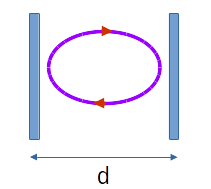
\includegraphics[scale=0.75]{optical_cavity.png}
\caption{Illustration of a basic optical cavity.}
\end{figure}

\section{Different Types of Optical Resonators}
\subsection{Fabry-Perot Resonator}
A system of two mirrors held parallel to each other and both having high reflectivity’s show a resonant behavior at some frequencies of the incident light. If both the mirrors have high reflectance, the incident light is still observed to pass through them without any decrease in the intensity and is detected, which occurs due to phenomenon’s similar to quantum tunneling effects [14].

\subsection{Gires-Tournois}
It is basically a lossless Fabry-Perot resonator which has a 100$\%$ reflecting rear mirror, that means it reflects 100$\%$ at all frequencies. Still, some resonant frequencies stay between the mirrors for a longer period of time and thus descript resonant behavior and lead to ultra slow group velocities. This simple device is known for storing spectral power of light which is reflected from it while modifying its phase. That is why it is sometimes referred to as a "phase only" filter.


\section{Micro Resonators}
Microresonators are a special type of resonators made from a different type of materials which exhibit optical properties while being fabricated on a chip [8]. These kinds of resonators are actually useful in observing the effects of optical resonators on a device.

\subsection{Different Geometeries}
There are many types of microresonators from which micro ring-resonators are very useful in making photonic devices and have a wide variety of application. Other kinds of resonators are also useful for different kind of applications and all have distinct optical properties based on their geometry. (See figure 1.2)
\begin{figure}[h]
\centering
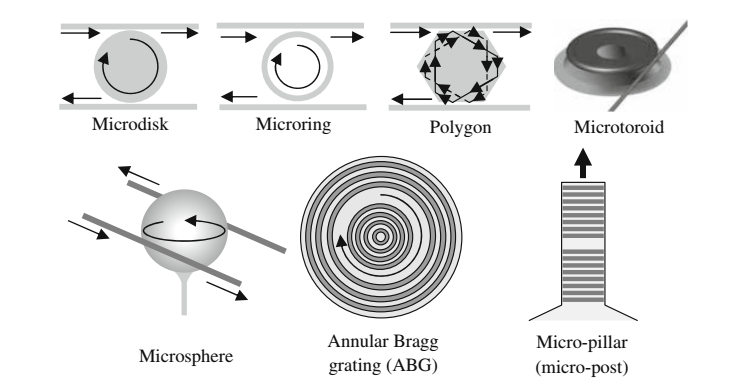
\includegraphics[width=1\textwidth]{microresonators_types.jpg}
\caption{Different geometries of microresonators.[15]}
\end{figure}


\section{Electromagnetically Induced Transparency and Absorption (EIT and EIA)}
Electromagnetically Induced Transparency (EIT) is a coherent optical nonlinearity which makes a medium transparent to some narrow bandwidth of frequencies which were otherwise opaque to the incident radiation. This window leads to slow light at resonant frequencies in an optical resonant system usually involving coupled system. This is observed due to the destructive quantum interference effects of the incident radiation in atomic levels [4].

\subparagraph{\normalfont \large Similarly, Electromagnetically Induced Absorption (EIA), is a similar phenomenon to EIT but in this nonlinearity, the medium becomes highly opaque to some bandwidth of frequencies at resonance. Thus blocking off completely the resonant frequency radiation and, causing a dip in the transmitted field. The quantum interference of light here is destructive and the atomic levels absorb the extra photons at such particular frequencies.[7]}

\section{Aims and Objectives}
This thesis is a detailed study of the optical properties of such photonic resonators which are composed of passive and active material. We deeply study the changing behavior of active and passive resonators in different parameters. Active resonators are those resonators which are made from some gain medium and they also descript EIT and EIA like behavior in a similar and distinct fashion. We hope to achieve gain controlled variation between slow and fast group velocities of light and enhance the transmission of the system. Different scientific tools and utilities, such as Wolfram Mathematica and Python 3.5, are used to model these conditions and produce results.


\newpage
\section*{References}
\addcontentsline{toc}{section}{References}

\paragraph{\normalfont \large $[1]$  Kaminow, I.P., Li, T., et al. Optical fiber telecommunications. 5th Edition. Academic Press, Elsevier, San Diego (2008). \\ 
\\$[2]$ A. Naweed, G. Farca, S. I. Shopova, and A. T. Rosenberger "Induced transparency and absorption in coupled whispering-gallery microresonators", Phys. Rev. A \textbf{71} (2005)\\
\\$[3]$ B. Peng1, S. K. Ozdemir, W. Chen, F. Nori, L. Yang "What is and what is not electromagnetically induced transparency in whispering-gallery microcavities", Nature. Comm. (2014). \\
\\$[4]$ John E. Heebner, Ph.D. Thesis, "Nonlinear Optical Whispering Gallery Microresonators for Photonics", (2003)  \\
\\$[5]$ K. J. Vahala, “Optical microcavities,” Nature \textbf{424} (2003).\\
\\$[6]$ L. Maleki, A. B. Matsko, A. A. Savchenkov, and V. S. Ilchenko, “Tunable delay line with interacting
whispering-gallery-mode resonators,” Opt. Lett. 29(6), 626–628 (2004).\\
\\$[7]$ A. Naweed, D. Goldberg, and V. M. Menon, “All-optical electromagnetically induced transparency using
coupled one-dimensional microcavities,” Opt. Express 22, 18818–18823 (2014).\\
\\$[8]$ M. Borselli, T. Johnson, and O. Painter, “Beyond the Rayleigh scattering limit in high-Q silicon microdisks:
theory and experiment,” Opt. Express 13(5), 1515–1530 (2005).\\
\\$[9]$ Kobrinsky, M. J., Block, B.A., et al. On-chip optical interconnects. Intel Technol. J. \textbf{8}, 129 (2004).\\
\\$[10]$ Barwicz, T., Byun, H., et al. Silicon photonics for compact, energy-efficient interconnects. J. Opt. Networking \textbf{6}, 63 (2007)\\
\\$[11]$ Ishikawa, H. Ultrafast all-optical signal processing devices. John Wiley and Sons, New Jersey (2008). \\
\\$[12]$ Xia, F., Sekaric, L., et al. Ultracompact optical buffers on a silicon chip. Nature \textbf{1}, 65–71
(2007).\\
\\$[13]$ Landobasa, Y.M., Chin, M.K. Optical buffer with higher delay-bandwidth product in a tworing system. Opt. Express \textbf{16}, 1796–1807 (2008).
\\$[14]$ Fabry, C., Pérot, A. Théorie et applications d’une nouvelle méthode de spectroscopie interférentielle. Ann. Chim. Phys. \textbf{16}, 115 (1899).\\
\\$[15]$ Vahala, K.J. Optical microcavities. Nature \textbf{424}, 839–846 (2003).\\
\\$[16]$ M. Bayindir, S. Tanriseven, A. Aydinli, and E. Ozbay, “Strong enhancement of spontaneous emission in
amorphous-silicon-nitride photonic crystal based coupled-microcavity structures,” Appl. Phys., A Mater. Sci.
Process. \textbf{73}(1), 125–127 (2001).\\
\\$[17]$ A. J. Campillo, J. D. Eversole, and H.-B. Lin, “Cavity quantum electrodynamic enhancement of stimulated
emission in microdroplets,” Phys. Rev. Lett. \textbf{67}(4), 437–440 (1991).\\
\\$[18]$ D. Gerace, H. E. Türeci, A. Imamoglu, V. Giovannetti, and R. Fazio, “The quantum-optical Josephson
interferometer,” Nat. Phys. \textbf{5}(4), 281–284 (2009).\\
\\$[19]$  C. Diederichs, J. Tignon, G. Dasbach, C. Ciuti, A. Lemaître, J. Bloch, P. Roussignol, and C. Delalande,
“Parametric oscillation in vertical triple microcavities,” Nature \textbf{440}(7086), 904–907 (2006).\\
\\$[20]$ Q. Xu, S. Sandhu, M. L. Povinelli, J. Shakya, S. Fan, and M. Lipson, “Experimental realization of an on-chip alloptical analogue to electromagnetically induced transparency,” Phys. Rev. Lett. \textbf{96}(12), 123901 (2006).}